% E04. Evolucion de las variables hidrologicas.
% Va en el dossier en lugar de la seccion E04 de la plantilla:
%   % E04. Evolucion de las variables hidrologicas.
% Va en el dossier en lugar de la seccion E04 de la plantilla:
%   % E04. Evolucion de las variables hidrologicas.
% Va en el dossier en lugar de la seccion E04 de la plantilla:
%   % E04. Evolucion de las variables hidrologicas.
% Va en el dossier en lugar de la seccion E04 de la plantilla:
%   \input{evidencias/E04_evolucion_variables}
% Cifras: 03_outputs/tables/05_estadisticos_anuales_E04.csv, 05_anios_extremos_E04.csv,
% 05_relaciones_anuales_E04.csv, 05_relleno_por_anio_E04.csv, 05_clima_caudal_anual.csv
% y 05_pettitt_clima_anual.csv, generadas por run_all.R.
% Periodo 1987-2019, poligono de Alexis, caudal rellenado.

\section{E04. Evolución de las variables hidrológicas}
\label{ev:E04}

\campo{1. Pregunta o afirmación que se evalúa}{¿Cómo varían la P, las
temperaturas, la PET y el caudal entre años en 1987--2019, y qué contrastes
son defendibles?}

\campo{2. Evidencia principal}{Las series anuales de P, PET y Q y de Tmax,
Tmed y Tmin (Figura~\ref{fig:E04evolucion}), sus estadísticos en el período
(Tabla~\ref{tab:E04estadisticos}), los tres años más secos y más húmedos
según la P (Tabla~\ref{tab:E04extremos}) y las relaciones entre variables
(Tabla~\ref{tab:E04relaciones}). Agregación por año calendario: P, PET y Q
se suman y las temperaturas se promedian; un año entra solo si tiene todos
sus días. Con el caudal rellenado (E02) entran los 33 años; ninguno se
excluye. La ET real y la demanda se tratan en E05 a E07.}

\begin{figure}[ht]
\centering
\IfFileExists{../03_outputs/figures/05_evolucion_anual.png}{%
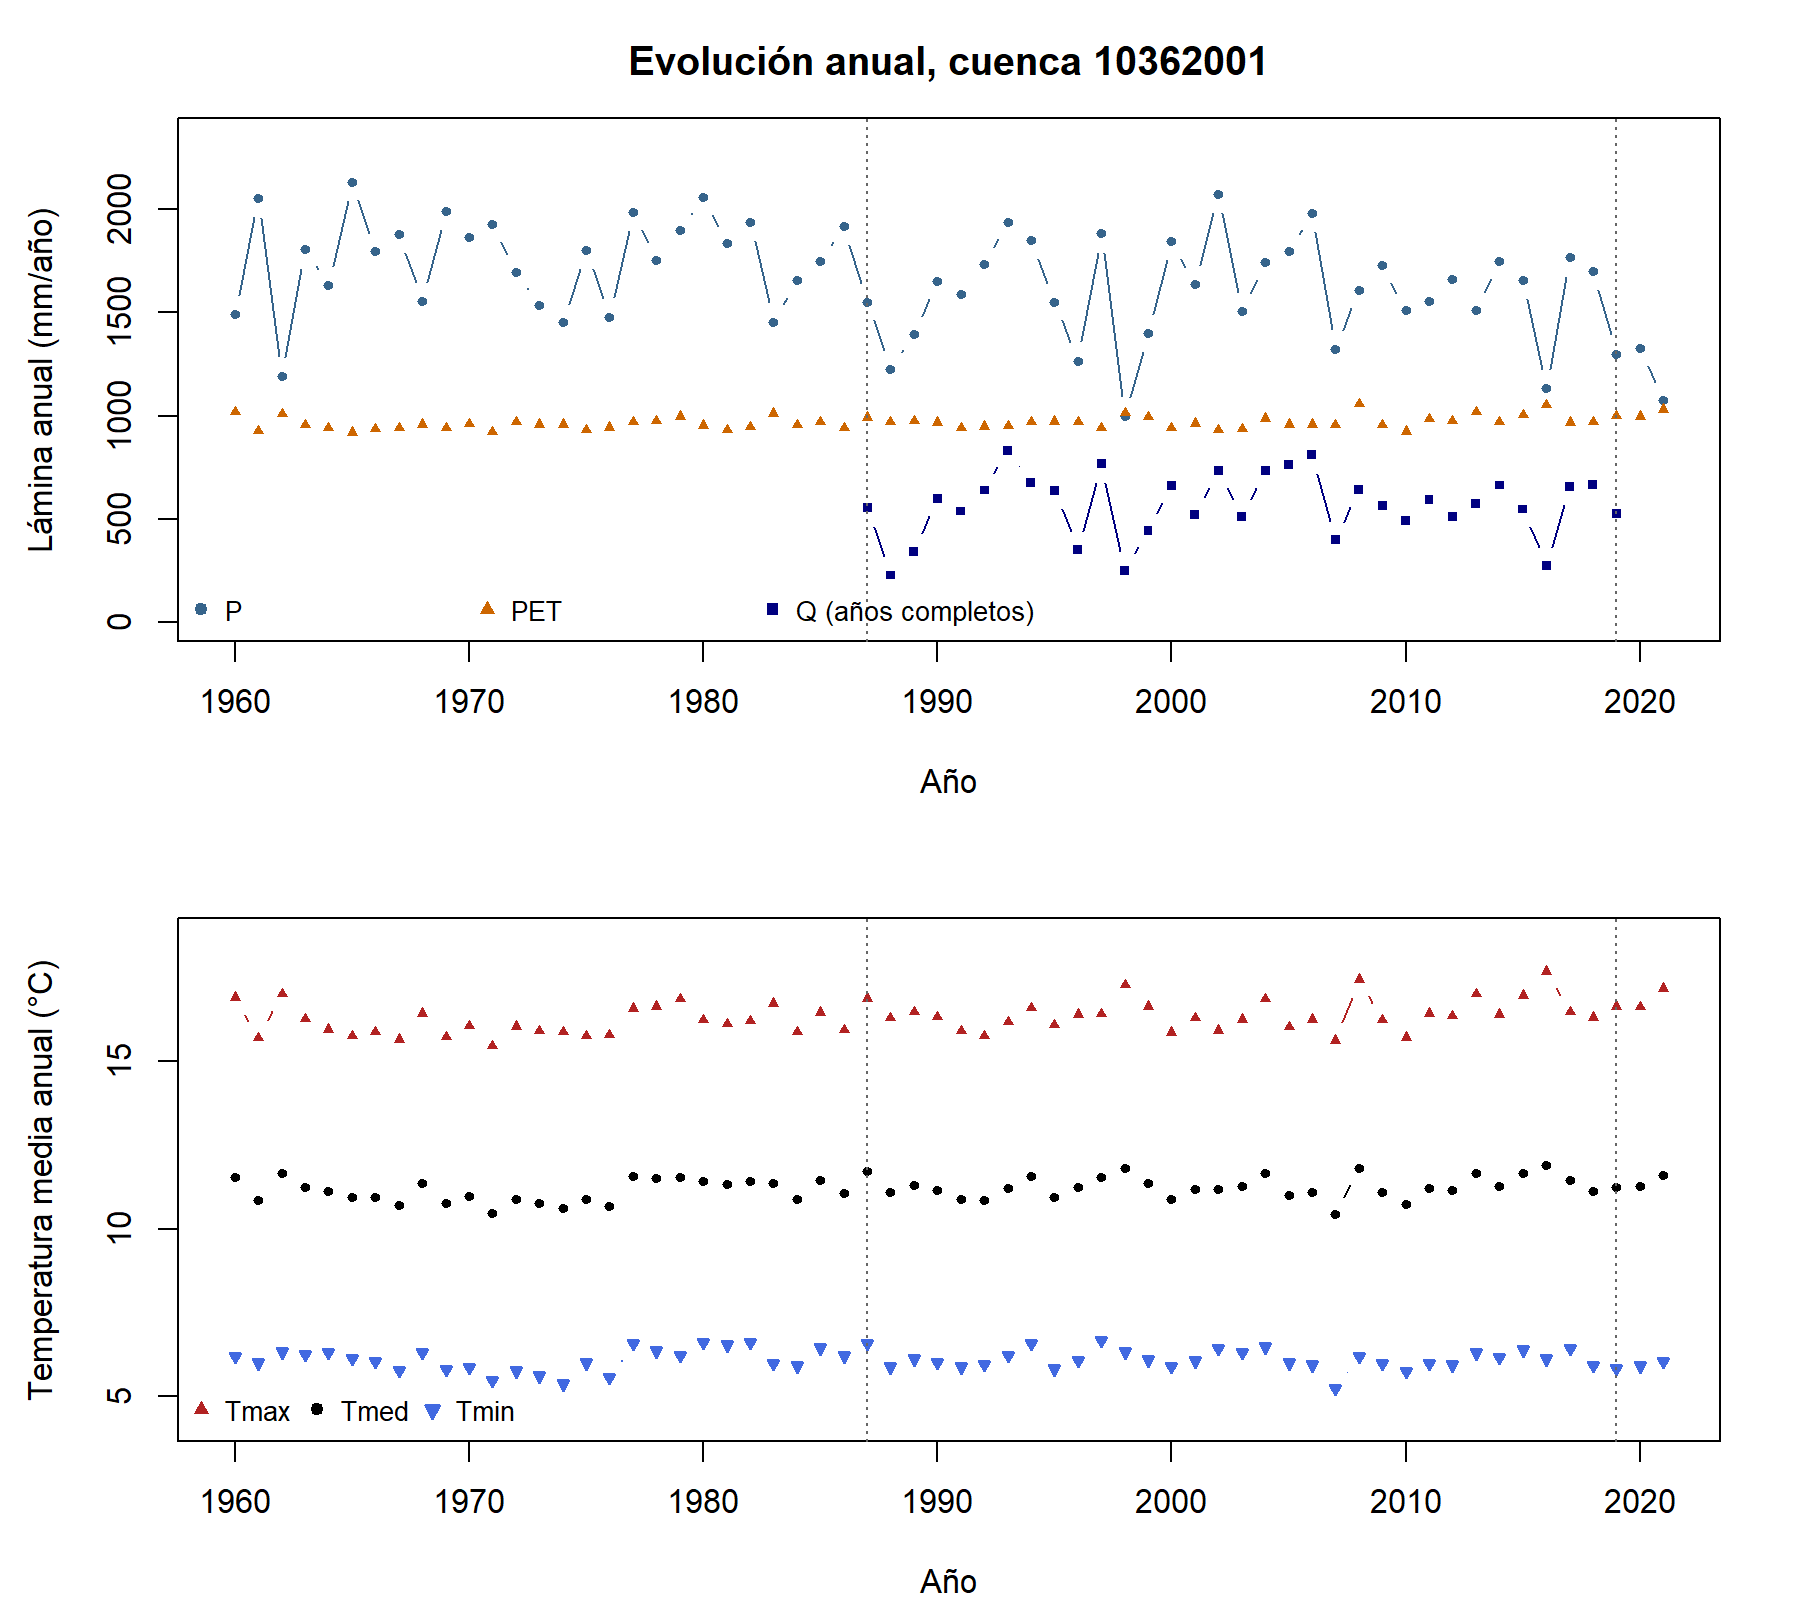
\includegraphics[width=0.9\textwidth]{../03_outputs/figures/05_evolucion_anual.png}}{%
\fbox{Falta 03\_outputs/figures/05\_evolucion\_anual.png}}
\caption{Arriba: P, PET y Q anuales en lámina (mm\,año$^{-1}$). Abajo:
Tmax, Tmed y Tmin anuales (°C). Clima de CR2MET v2.5 \citep{Boisier2023} de
1960 a 2021; caudal DGA rellenado de 1987 a 2019. Las líneas punteadas
marcan el período de análisis.}
\label{fig:E04evolucion}
\end{figure}

\begin{table}[ht]
\centering
\caption{Estadísticos anuales, 1987--2019 (33 años). CV: coeficiente de
variación. Q/P es adimensional.}
\label{tab:E04estadisticos}
\begin{tabular}{|p{0.22\linewidth}|r|r|r|r|r|}
\hline
Variable & Media & Desviación & CV (\%) & Mínimo (año) & Máximo (año) \\
\hline
P (mm\,año$^{-1}$) & 1601.6 & 247.9 & 15.5 & 999.6 (1998) & 2075.6 (2002) \\
\hline
PET (mm\,año$^{-1}$) & 973.4 & 31.1 & 3.2 & 923.6 (2010) & 1057.8 (2008) \\
\hline
Q (mm\,año$^{-1}$) & 566.1 & 157.2 & 27.8 & 226.7 (1988) & 832.1 (1993) \\
\hline
Q medio (m$^3$\,s$^{-1}$) & 8.41 & 2.34 & 27.8 & 3.36 (1988) & 12.37 (1993) \\
\hline
Q/P & 0.35 & 0.06 & 17.0 & 0.18 (1988) & 0.43 (1993) \\
\hline
Tmax (°C) & 16.43 & 0.48 & 2.9 & 15.62 (2007) & 17.69 (2016) \\
\hline
Tmed (°C) & 11.27 & 0.34 & 3.0 & 10.43 (2007) & 11.91 (2016) \\
\hline
Tmin (°C) & 6.11 & 0.29 & 4.7 & 5.24 (2007) & 6.68 (1997) \\
\hline
\end{tabular}
\end{table}

\begin{table}[ht]
\centering
\caption{Los tres años más secos y los tres más húmedos según la P,
1987--2019. P, PET y Q en mm\,año$^{-1}$; Q/P adimensional.}
\label{tab:E04extremos}
\begin{tabular}{|l|l|r|r|r|r|}
\hline
Tipo & Año & P & PET & Q & Q/P \\
\hline
Seco & 1998 & 999.6 & 1013.2 & 248.9 & 0.25 \\
\hline
Seco & 2016 & 1132.4 & 1053.7 & 272.6 & 0.24 \\
\hline
Seco & 1988 & 1227.5 & 970.8 & 226.7 & 0.18 \\
\hline
Húmedo & 1993 & 1938.8 & 952.1 & 832.1 & 0.43 \\
\hline
Húmedo & 2006 & 1984.1 & 958.1 & 810.3 & 0.41 \\
\hline
Húmedo & 2002 & 2075.6 & 932.6 & 733.9 & 0.35 \\
\hline
\end{tabular}
\end{table}

\begin{table}[ht]
\centering
\caption{Relaciones entre variables anuales, 1987--2019 (33 años).}
\label{tab:E04relaciones}
\begin{tabular}{|p{0.55\linewidth}|r|}
\hline
Indicador & Valor \\
\hline
Correlación de P y Q anuales & 0.92 \\
\hline
Correlación de P y PET anuales & $-$0.49 \\
\hline
Correlación de PET y Tmed anuales & 0.72 \\
\hline
P $-$ Q medio, ecuación~(\ref{eq:E04balance}) (mm\,año$^{-1}$) & 1035.4 \\
\hline
PET media (mm\,año$^{-1}$) & 973.4 \\
\hline
(P $-$ Q)/PET & 1.064 \\
\hline
Años con P $-$ Q mayor que la PET & 23 de 33 \\
\hline
Volumen anual que viene de días rellenados, 2016 / 2013 & 45.0 / 44.3 \% \\
\hline
\end{tabular}
\end{table}

\campo{3. Fuente y trazabilidad}{Las series anuales salen de
\texttt{02\_\allowbreak{}Rscripts/\allowbreak{}05\_\allowbreak{}regimen\_\allowbreak{}hidroclimatico.R}, que agrega la serie
diaria de clima de E02 y el caudal rellenado pasado a lámina con el área de
E01 (468.73 km$^2$). Las cifras de esta ficha están en
\texttt{03\_\allowbreak{}outputs/\allowbreak{}tables/\allowbreak{}} (\texttt{05\_\allowbreak{}clima\_\allowbreak{}caudal\_\allowbreak{}anual.csv},
\texttt{05\_\allowbreak{}estadisticos\_\allowbreak{}anuales\_\allowbreak{}E04.csv},
\texttt{05\_\allowbreak{}anios\_\allowbreak{}extremos\_\allowbreak{}E04.csv},
\texttt{05\_\allowbreak{}relaciones\_\allowbreak{}anuales\_\allowbreak{}E04.csv} y
\texttt{05\_\allowbreak{}relleno\_\allowbreak{}por\_\allowbreak{}anio\_\allowbreak{}E04.csv}) y la figura en
\texttt{03\_\allowbreak{}outputs/\allowbreak{}figures/\allowbreak{}05\_\allowbreak{}evolucion\_\allowbreak{}anual.png}. El período se lee de
\texttt{06\_\allowbreak{}config/\allowbreak{}parametros.csv}, las fuentes están en
\texttt{04\_\allowbreak{}metadata/\allowbreak{}data\_\allowbreak{}sources.csv} y todo se regenera con
\texttt{run\_\allowbreak{}all.R}.}

\campo{4. Interpretación hidrológica}{El caudal varía casi el doble que la
lluvia: su coeficiente de variación es 27.8 \%, contra 15.5 \% de la
P. La correlación entre P y Q anuales es 0.92, pero la respuesta no es
proporcional. En los años secos solo entre un 18 y un
25 \% de la P sale como caudal, y en los húmedos llega hasta un
43 \%: con menos lluvia, la parte que se evapora o queda en la
cuenca pesa más. La PET casi no cambia entre años (CV 3.2 \%) y tiende
a ir al revés de la P (correlación $-$0.49): 1998 y 2016, dos de los años
más secos, tienen PET sobre la media, aunque 1988 no. La ecuación de
Hargreaves hace subir la PET con la temperatura y con la diferencia entre
Tmax y Tmin, que está ligada a la nubosidad \citep{Allen1998}. Las
temperaturas varían poco: la Tmed va de 10.43 °C (2007) a
11.91 °C (2016).

En 1987--2019 no se detecta un cambio en P, PET ni Tmed: Pettitt no
encuentra quiebre y el KPSS no rechaza la estacionariedad, aunque el ADF no
la confirma (E02). Las pruebas del integrante 2 tampoco encuentran quiebre en
el caudal. No se aplicó una prueba de tendencia, así que lo defendible es que
no se detecta cambio, no que no lo haya. En el registro largo sí hay cambios:
el de Tmed (desde 1977) es anterior al período, el de P (desde 1987) coincide
con su inicio, y el de PET (desde 2011, +3.8 \%) cae dentro del período, pero
dentro de 1987--2019 no resulta significativo.}

\campo{5. Consistencia física}{Los flujos se suman en el año y las
temperaturas se promedian; los años bisiestos entran con sus 366 días porque
la regla de completitud cuenta los días del calendario. El caudal en lámina
sale de la ecuación~(\ref{eq:E03lamina}) de E03, sumada en el año. Si el
almacenamiento no cambia en el largo plazo, la ET real es lo que queda del
balance:
\begin{equation}
\mathrm{ET}_{\mathrm{real}} \approx P - Q
\label{eq:E04balance}
\end{equation}
Aquí P $-$ Q supera a la PET en un 6.4 \% en promedio y en
23 de los 33 años (Tabla~\ref{tab:E04relaciones}). La PET de
Hargreaves estima la ET de un cultivo de referencia \citep{Allen1998} y no
la de la cobertura real de la cuenca, pero un exceso sostenido indica además
que algún término puede tener un sesgo: la P sobreestimada, el caudal
subestimado (extracciones, pérdidas hacia el acuífero o la curva de
descarga) o la PET subestimada. Se trata en E05 y E06.}

\campo{6. Limitaciones e incertidumbre}{33 años es poco para hablar de
tendencias. En 11 de los 33 años el caudal anual incluye días rellenados
(E02), con bloques de hasta 71 días. En 2016, uno de los años más secos, el
45.0 \% del volumen anual viene de días rellenados, y en 2013 el
44.3 \%, así que el Q/P de esos años depende en buena parte de la
regresión. En 2014 los 15 días rellenados quedaron en 0 y no aportan
volumen. La P, Tmax y Tmin son de un producto grillado y la PET de una
fórmula que usa solo temperatura, así que la relación entre PET y P refleja
también cómo se construyen esas variables.}

\campo{7. Conclusión asociada}{Entre 1987 y 2019 el caudal del Río Damas en
Tacamo varía casi el doble que la lluvia y responde a ella de forma no
proporcional: en los años secos sale como caudal una fracción menor de la P.
En el período no se detecta cambio en P, PET, Tmed ni Q. El balance de largo
plazo deja P $-$ Q por encima de la PET en 23 de 33 años, algo que E05 y E06
tienen que explicar antes de interpretar la ET real.}

% Cifras: 03_outputs/tables/05_estadisticos_anuales_E04.csv, 05_anios_extremos_E04.csv,
% 05_relaciones_anuales_E04.csv, 05_relleno_por_anio_E04.csv, 05_clima_caudal_anual.csv
% y 05_pettitt_clima_anual.csv, generadas por run_all.R.
% Periodo 1987-2019, poligono de Alexis, caudal rellenado.

\section{E04. Evolución de las variables hidrológicas}
\label{ev:E04}

\campo{1. Pregunta o afirmación que se evalúa}{¿Cómo varían la P, las
temperaturas, la PET y el caudal entre años en 1987--2019, y qué contrastes
son defendibles?}

\campo{2. Evidencia principal}{Las series anuales de P, PET y Q y de Tmax,
Tmed y Tmin (Figura~\ref{fig:E04evolucion}), sus estadísticos en el período
(Tabla~\ref{tab:E04estadisticos}), los tres años más secos y más húmedos
según la P (Tabla~\ref{tab:E04extremos}) y las relaciones entre variables
(Tabla~\ref{tab:E04relaciones}). Agregación por año calendario: P, PET y Q
se suman y las temperaturas se promedian; un año entra solo si tiene todos
sus días. Con el caudal rellenado (E02) entran los 33 años; ninguno se
excluye. La ET real y la demanda se tratan en E05 a E07.}

\begin{figure}[ht]
\centering
\IfFileExists{../03_outputs/figures/05_evolucion_anual.png}{%
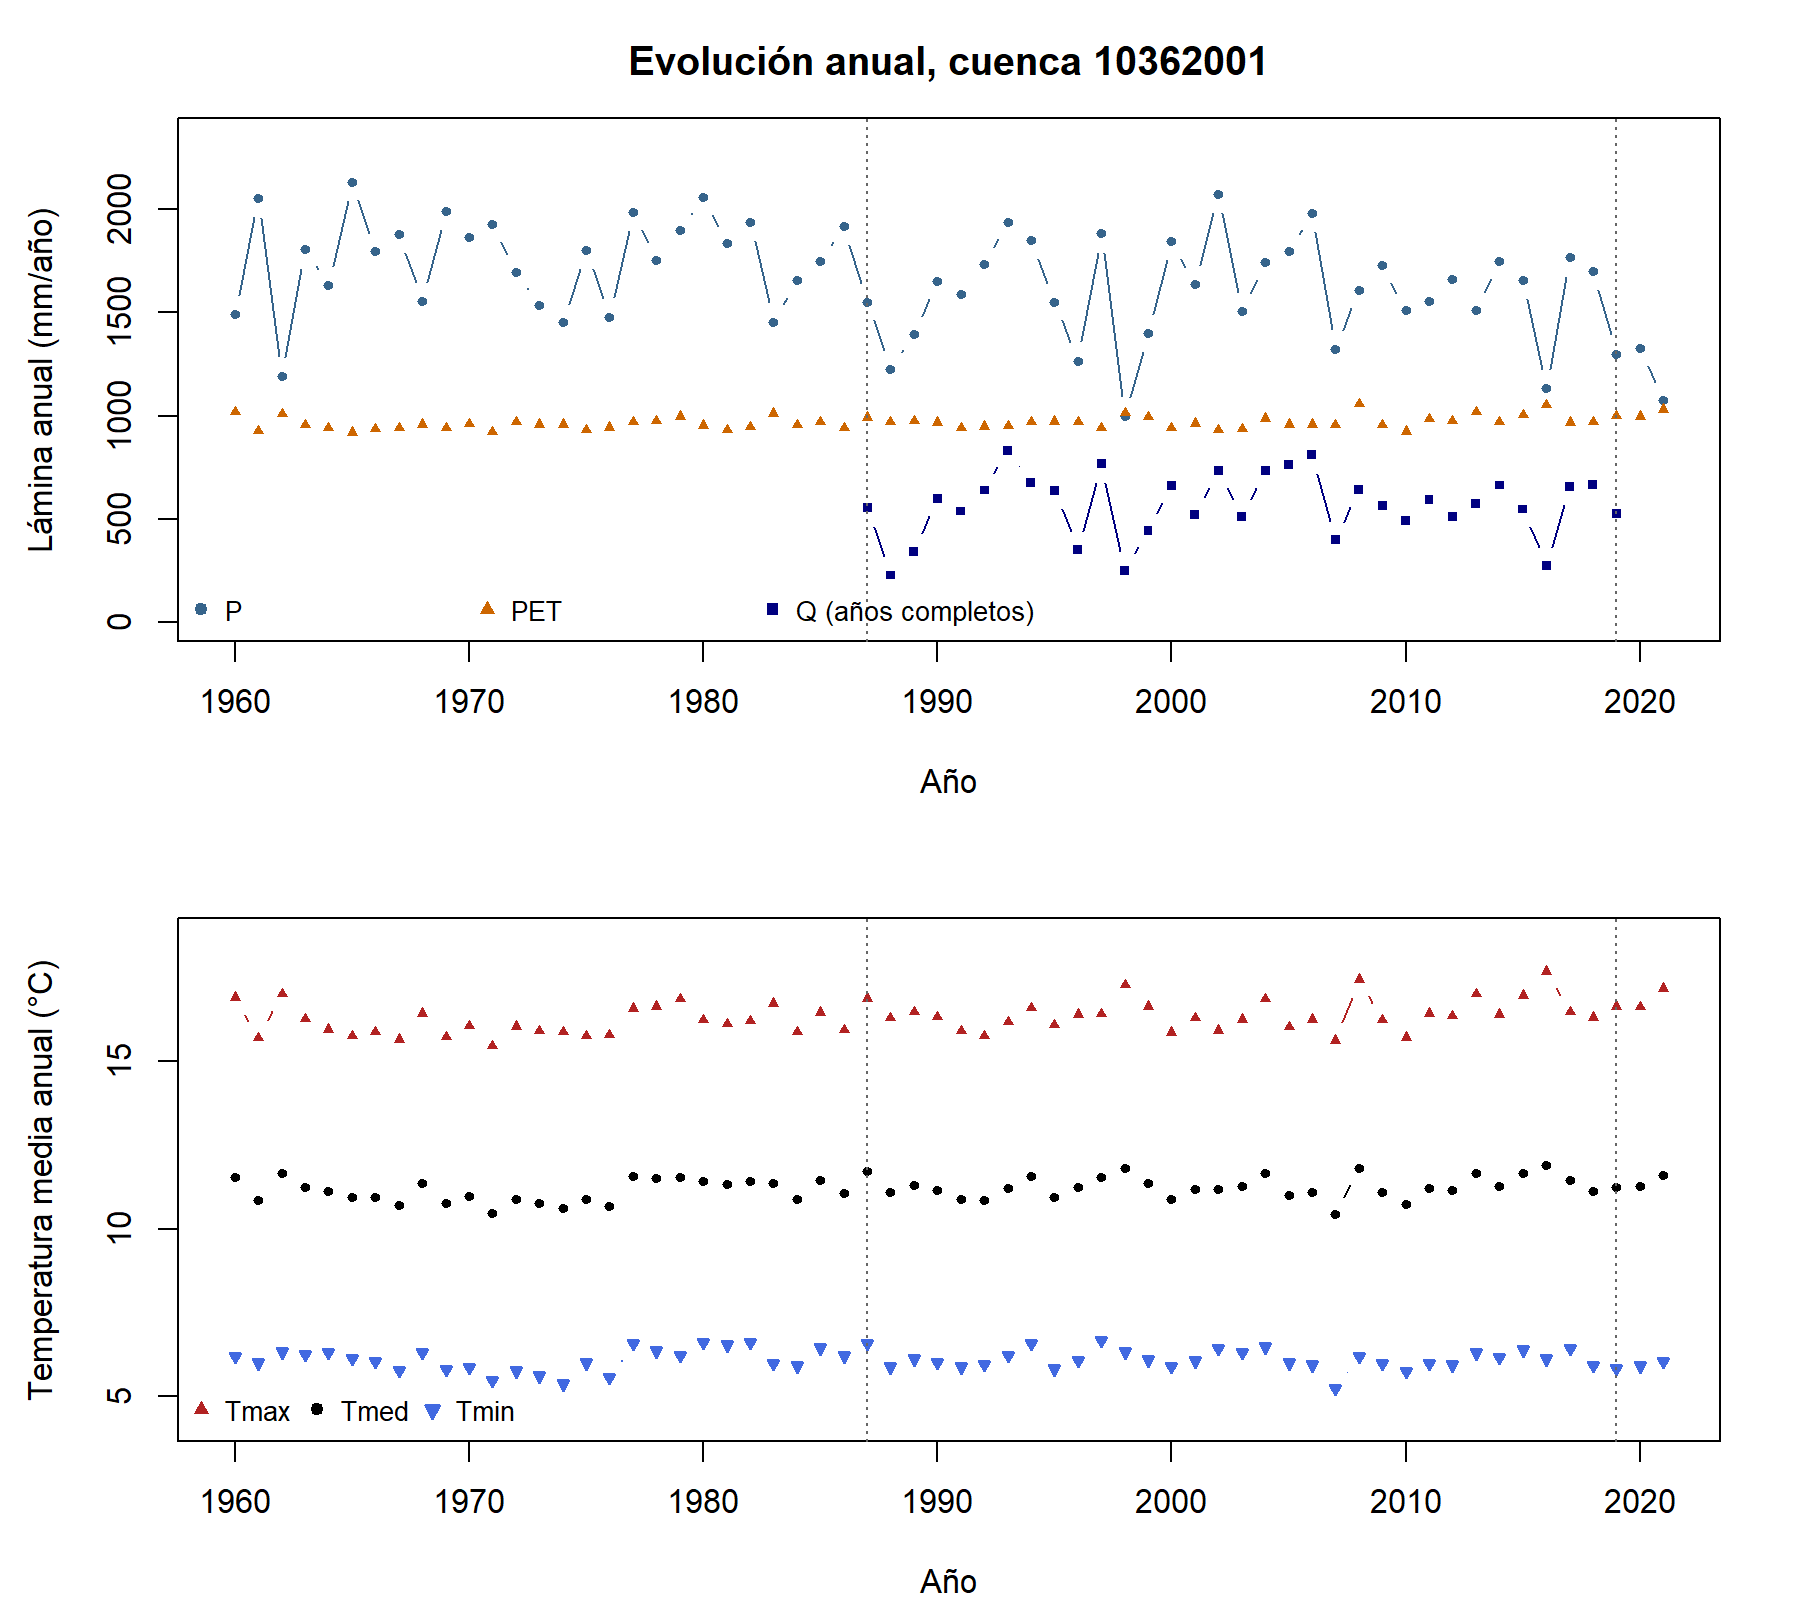
\includegraphics[width=0.9\textwidth]{../03_outputs/figures/05_evolucion_anual.png}}{%
\fbox{Falta 03\_outputs/figures/05\_evolucion\_anual.png}}
\caption{Arriba: P, PET y Q anuales en lámina (mm\,año$^{-1}$). Abajo:
Tmax, Tmed y Tmin anuales (°C). Clima de CR2MET v2.5 \citep{Boisier2023} de
1960 a 2021; caudal DGA rellenado de 1987 a 2019. Las líneas punteadas
marcan el período de análisis.}
\label{fig:E04evolucion}
\end{figure}

\begin{table}[ht]
\centering
\caption{Estadísticos anuales, 1987--2019 (33 años). CV: coeficiente de
variación. Q/P es adimensional.}
\label{tab:E04estadisticos}
\begin{tabular}{|p{0.22\linewidth}|r|r|r|r|r|}
\hline
Variable & Media & Desviación & CV (\%) & Mínimo (año) & Máximo (año) \\
\hline
P (mm\,año$^{-1}$) & 1601.6 & 247.9 & 15.5 & 999.6 (1998) & 2075.6 (2002) \\
\hline
PET (mm\,año$^{-1}$) & 973.4 & 31.1 & 3.2 & 923.6 (2010) & 1057.8 (2008) \\
\hline
Q (mm\,año$^{-1}$) & 566.1 & 157.2 & 27.8 & 226.7 (1988) & 832.1 (1993) \\
\hline
Q medio (m$^3$\,s$^{-1}$) & 8.41 & 2.34 & 27.8 & 3.36 (1988) & 12.37 (1993) \\
\hline
Q/P & 0.35 & 0.06 & 17.0 & 0.18 (1988) & 0.43 (1993) \\
\hline
Tmax (°C) & 16.43 & 0.48 & 2.9 & 15.62 (2007) & 17.69 (2016) \\
\hline
Tmed (°C) & 11.27 & 0.34 & 3.0 & 10.43 (2007) & 11.91 (2016) \\
\hline
Tmin (°C) & 6.11 & 0.29 & 4.7 & 5.24 (2007) & 6.68 (1997) \\
\hline
\end{tabular}
\end{table}

\begin{table}[ht]
\centering
\caption{Los tres años más secos y los tres más húmedos según la P,
1987--2019. P, PET y Q en mm\,año$^{-1}$; Q/P adimensional.}
\label{tab:E04extremos}
\begin{tabular}{|l|l|r|r|r|r|}
\hline
Tipo & Año & P & PET & Q & Q/P \\
\hline
Seco & 1998 & 999.6 & 1013.2 & 248.9 & 0.25 \\
\hline
Seco & 2016 & 1132.4 & 1053.7 & 272.6 & 0.24 \\
\hline
Seco & 1988 & 1227.5 & 970.8 & 226.7 & 0.18 \\
\hline
Húmedo & 1993 & 1938.8 & 952.1 & 832.1 & 0.43 \\
\hline
Húmedo & 2006 & 1984.1 & 958.1 & 810.3 & 0.41 \\
\hline
Húmedo & 2002 & 2075.6 & 932.6 & 733.9 & 0.35 \\
\hline
\end{tabular}
\end{table}

\begin{table}[ht]
\centering
\caption{Relaciones entre variables anuales, 1987--2019 (33 años).}
\label{tab:E04relaciones}
\begin{tabular}{|p{0.55\linewidth}|r|}
\hline
Indicador & Valor \\
\hline
Correlación de P y Q anuales & 0.92 \\
\hline
Correlación de P y PET anuales & $-$0.49 \\
\hline
Correlación de PET y Tmed anuales & 0.72 \\
\hline
P $-$ Q medio, ecuación~(\ref{eq:E04balance}) (mm\,año$^{-1}$) & 1035.4 \\
\hline
PET media (mm\,año$^{-1}$) & 973.4 \\
\hline
(P $-$ Q)/PET & 1.064 \\
\hline
Años con P $-$ Q mayor que la PET & 23 de 33 \\
\hline
Volumen anual que viene de días rellenados, 2016 / 2013 & 45.0 / 44.3 \% \\
\hline
\end{tabular}
\end{table}

\campo{3. Fuente y trazabilidad}{Las series anuales salen de
\texttt{02\_\allowbreak{}Rscripts/\allowbreak{}05\_\allowbreak{}regimen\_\allowbreak{}hidroclimatico.R}, que agrega la serie
diaria de clima de E02 y el caudal rellenado pasado a lámina con el área de
E01 (468.73 km$^2$). Las cifras de esta ficha están en
\texttt{03\_\allowbreak{}outputs/\allowbreak{}tables/\allowbreak{}} (\texttt{05\_\allowbreak{}clima\_\allowbreak{}caudal\_\allowbreak{}anual.csv},
\texttt{05\_\allowbreak{}estadisticos\_\allowbreak{}anuales\_\allowbreak{}E04.csv},
\texttt{05\_\allowbreak{}anios\_\allowbreak{}extremos\_\allowbreak{}E04.csv},
\texttt{05\_\allowbreak{}relaciones\_\allowbreak{}anuales\_\allowbreak{}E04.csv} y
\texttt{05\_\allowbreak{}relleno\_\allowbreak{}por\_\allowbreak{}anio\_\allowbreak{}E04.csv}) y la figura en
\texttt{03\_\allowbreak{}outputs/\allowbreak{}figures/\allowbreak{}05\_\allowbreak{}evolucion\_\allowbreak{}anual.png}. El período se lee de
\texttt{06\_\allowbreak{}config/\allowbreak{}parametros.csv}, las fuentes están en
\texttt{04\_\allowbreak{}metadata/\allowbreak{}data\_\allowbreak{}sources.csv} y todo se regenera con
\texttt{run\_\allowbreak{}all.R}.}

\campo{4. Interpretación hidrológica}{El caudal varía casi el doble que la
lluvia: su coeficiente de variación es 27.8 \%, contra 15.5 \% de la
P. La correlación entre P y Q anuales es 0.92, pero la respuesta no es
proporcional. En los años secos solo entre un 18 y un
25 \% de la P sale como caudal, y en los húmedos llega hasta un
43 \%: con menos lluvia, la parte que se evapora o queda en la
cuenca pesa más. La PET casi no cambia entre años (CV 3.2 \%) y tiende
a ir al revés de la P (correlación $-$0.49): 1998 y 2016, dos de los años
más secos, tienen PET sobre la media, aunque 1988 no. La ecuación de
Hargreaves hace subir la PET con la temperatura y con la diferencia entre
Tmax y Tmin, que está ligada a la nubosidad \citep{Allen1998}. Las
temperaturas varían poco: la Tmed va de 10.43 °C (2007) a
11.91 °C (2016).

En 1987--2019 no se detecta un cambio en P, PET ni Tmed: Pettitt no
encuentra quiebre y el KPSS no rechaza la estacionariedad, aunque el ADF no
la confirma (E02). Las pruebas del integrante 2 tampoco encuentran quiebre en
el caudal. No se aplicó una prueba de tendencia, así que lo defendible es que
no se detecta cambio, no que no lo haya. En el registro largo sí hay cambios:
el de Tmed (desde 1977) es anterior al período, el de P (desde 1987) coincide
con su inicio, y el de PET (desde 2011, +3.8 \%) cae dentro del período, pero
dentro de 1987--2019 no resulta significativo.}

\campo{5. Consistencia física}{Los flujos se suman en el año y las
temperaturas se promedian; los años bisiestos entran con sus 366 días porque
la regla de completitud cuenta los días del calendario. El caudal en lámina
sale de la ecuación~(\ref{eq:E03lamina}) de E03, sumada en el año. Si el
almacenamiento no cambia en el largo plazo, la ET real es lo que queda del
balance:
\begin{equation}
\mathrm{ET}_{\mathrm{real}} \approx P - Q
\label{eq:E04balance}
\end{equation}
Aquí P $-$ Q supera a la PET en un 6.4 \% en promedio y en
23 de los 33 años (Tabla~\ref{tab:E04relaciones}). La PET de
Hargreaves estima la ET de un cultivo de referencia \citep{Allen1998} y no
la de la cobertura real de la cuenca, pero un exceso sostenido indica además
que algún término puede tener un sesgo: la P sobreestimada, el caudal
subestimado (extracciones, pérdidas hacia el acuífero o la curva de
descarga) o la PET subestimada. Se trata en E05 y E06.}

\campo{6. Limitaciones e incertidumbre}{33 años es poco para hablar de
tendencias. En 11 de los 33 años el caudal anual incluye días rellenados
(E02), con bloques de hasta 71 días. En 2016, uno de los años más secos, el
45.0 \% del volumen anual viene de días rellenados, y en 2013 el
44.3 \%, así que el Q/P de esos años depende en buena parte de la
regresión. En 2014 los 15 días rellenados quedaron en 0 y no aportan
volumen. La P, Tmax y Tmin son de un producto grillado y la PET de una
fórmula que usa solo temperatura, así que la relación entre PET y P refleja
también cómo se construyen esas variables.}

\campo{7. Conclusión asociada}{Entre 1987 y 2019 el caudal del Río Damas en
Tacamo varía casi el doble que la lluvia y responde a ella de forma no
proporcional: en los años secos sale como caudal una fracción menor de la P.
En el período no se detecta cambio en P, PET, Tmed ni Q. El balance de largo
plazo deja P $-$ Q por encima de la PET en 23 de 33 años, algo que E05 y E06
tienen que explicar antes de interpretar la ET real.}

% Cifras: 03_outputs/tables/05_estadisticos_anuales_E04.csv, 05_anios_extremos_E04.csv,
% 05_relaciones_anuales_E04.csv, 05_relleno_por_anio_E04.csv, 05_clima_caudal_anual.csv
% y 05_pettitt_clima_anual.csv, generadas por run_all.R.
% Periodo 1987-2019, poligono de Alexis, caudal rellenado.

\section{E04. Evolución de las variables hidrológicas}
\label{ev:E04}

\campo{1. Pregunta o afirmación que se evalúa}{¿Cómo varían la P, las
temperaturas, la PET y el caudal entre años en 1987--2019, y qué contrastes
son defendibles?}

\campo{2. Evidencia principal}{Las series anuales de P, PET y Q y de Tmax,
Tmed y Tmin (Figura~\ref{fig:E04evolucion}), sus estadísticos en el período
(Tabla~\ref{tab:E04estadisticos}), los tres años más secos y más húmedos
según la P (Tabla~\ref{tab:E04extremos}) y las relaciones entre variables
(Tabla~\ref{tab:E04relaciones}). Agregación por año calendario: P, PET y Q
se suman y las temperaturas se promedian; un año entra solo si tiene todos
sus días. Con el caudal rellenado (E02) entran los 33 años; ninguno se
excluye. La ET real y la demanda se tratan en E05 a E07.}

\begin{figure}[ht]
\centering
\IfFileExists{../03_outputs/figures/05_evolucion_anual.png}{%
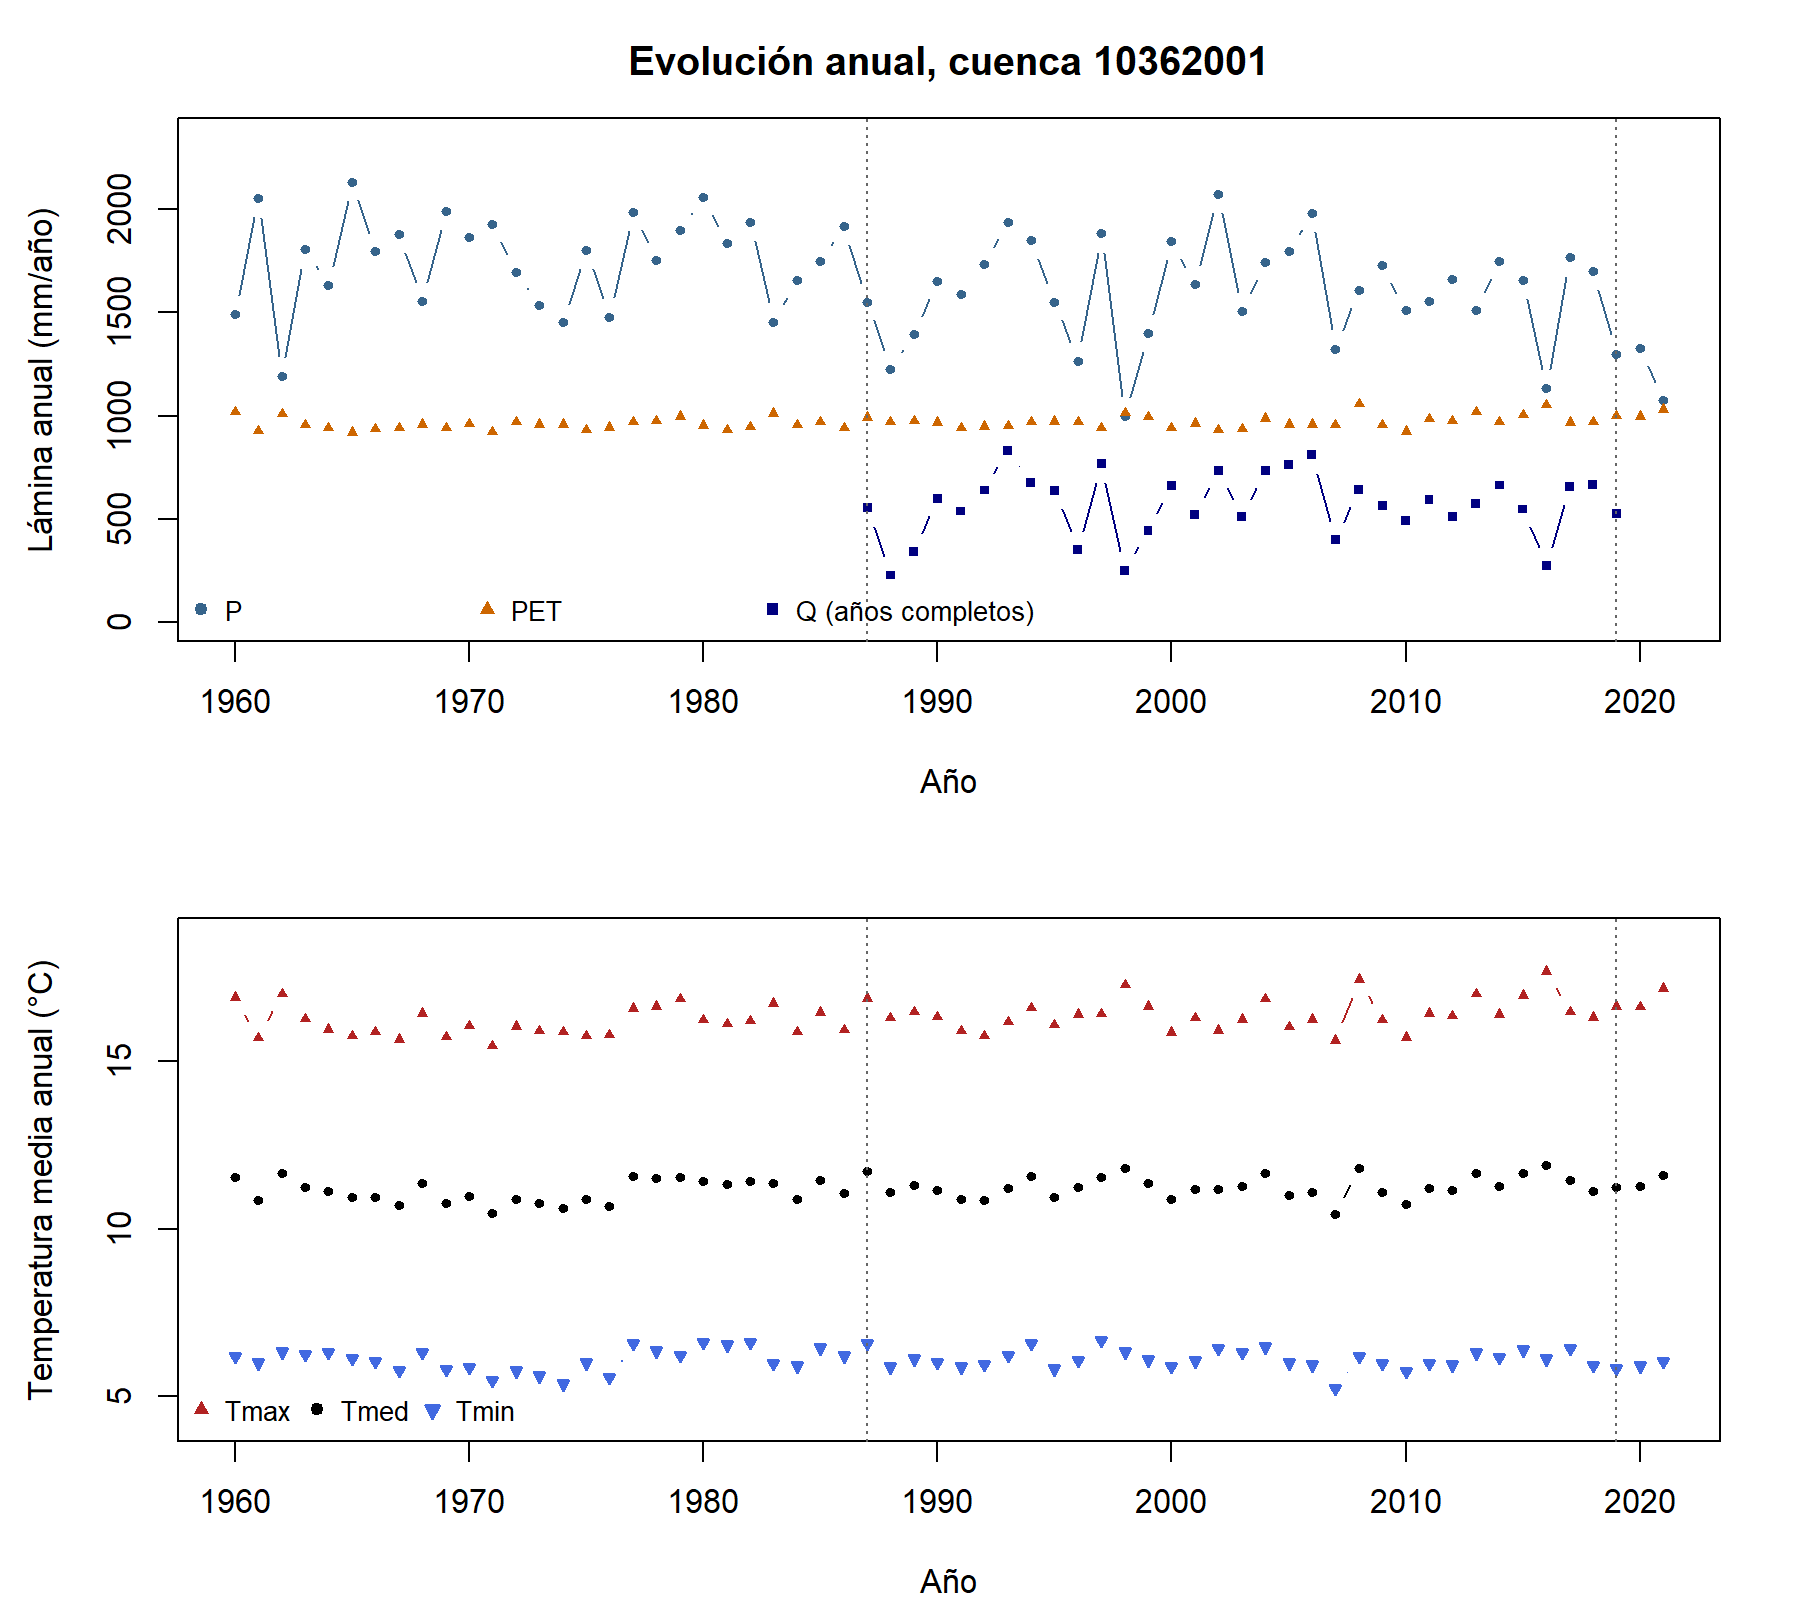
\includegraphics[width=0.9\textwidth]{../03_outputs/figures/05_evolucion_anual.png}}{%
\fbox{Falta 03\_outputs/figures/05\_evolucion\_anual.png}}
\caption{Arriba: P, PET y Q anuales en lámina (mm\,año$^{-1}$). Abajo:
Tmax, Tmed y Tmin anuales (°C). Clima de CR2MET v2.5 \citep{Boisier2023} de
1960 a 2021; caudal DGA rellenado de 1987 a 2019. Las líneas punteadas
marcan el período de análisis.}
\label{fig:E04evolucion}
\end{figure}

\begin{table}[ht]
\centering
\caption{Estadísticos anuales, 1987--2019 (33 años). CV: coeficiente de
variación. Q/P es adimensional.}
\label{tab:E04estadisticos}
\begin{tabular}{|p{0.22\linewidth}|r|r|r|r|r|}
\hline
Variable & Media & Desviación & CV (\%) & Mínimo (año) & Máximo (año) \\
\hline
P (mm\,año$^{-1}$) & 1601.6 & 247.9 & 15.5 & 999.6 (1998) & 2075.6 (2002) \\
\hline
PET (mm\,año$^{-1}$) & 973.4 & 31.1 & 3.2 & 923.6 (2010) & 1057.8 (2008) \\
\hline
Q (mm\,año$^{-1}$) & 566.1 & 157.2 & 27.8 & 226.7 (1988) & 832.1 (1993) \\
\hline
Q medio (m$^3$\,s$^{-1}$) & 8.41 & 2.34 & 27.8 & 3.36 (1988) & 12.37 (1993) \\
\hline
Q/P & 0.35 & 0.06 & 17.0 & 0.18 (1988) & 0.43 (1993) \\
\hline
Tmax (°C) & 16.43 & 0.48 & 2.9 & 15.62 (2007) & 17.69 (2016) \\
\hline
Tmed (°C) & 11.27 & 0.34 & 3.0 & 10.43 (2007) & 11.91 (2016) \\
\hline
Tmin (°C) & 6.11 & 0.29 & 4.7 & 5.24 (2007) & 6.68 (1997) \\
\hline
\end{tabular}
\end{table}

\begin{table}[ht]
\centering
\caption{Los tres años más secos y los tres más húmedos según la P,
1987--2019. P, PET y Q en mm\,año$^{-1}$; Q/P adimensional.}
\label{tab:E04extremos}
\begin{tabular}{|l|l|r|r|r|r|}
\hline
Tipo & Año & P & PET & Q & Q/P \\
\hline
Seco & 1998 & 999.6 & 1013.2 & 248.9 & 0.25 \\
\hline
Seco & 2016 & 1132.4 & 1053.7 & 272.6 & 0.24 \\
\hline
Seco & 1988 & 1227.5 & 970.8 & 226.7 & 0.18 \\
\hline
Húmedo & 1993 & 1938.8 & 952.1 & 832.1 & 0.43 \\
\hline
Húmedo & 2006 & 1984.1 & 958.1 & 810.3 & 0.41 \\
\hline
Húmedo & 2002 & 2075.6 & 932.6 & 733.9 & 0.35 \\
\hline
\end{tabular}
\end{table}

\begin{table}[ht]
\centering
\caption{Relaciones entre variables anuales, 1987--2019 (33 años).}
\label{tab:E04relaciones}
\begin{tabular}{|p{0.55\linewidth}|r|}
\hline
Indicador & Valor \\
\hline
Correlación de P y Q anuales & 0.92 \\
\hline
Correlación de P y PET anuales & $-$0.49 \\
\hline
Correlación de PET y Tmed anuales & 0.72 \\
\hline
P $-$ Q medio, ecuación~(\ref{eq:E04balance}) (mm\,año$^{-1}$) & 1035.4 \\
\hline
PET media (mm\,año$^{-1}$) & 973.4 \\
\hline
(P $-$ Q)/PET & 1.064 \\
\hline
Años con P $-$ Q mayor que la PET & 23 de 33 \\
\hline
Volumen anual que viene de días rellenados, 2016 / 2013 & 45.0 / 44.3 \% \\
\hline
\end{tabular}
\end{table}

\campo{3. Fuente y trazabilidad}{Las series anuales salen de
\texttt{02\_\allowbreak{}Rscripts/\allowbreak{}05\_\allowbreak{}regimen\_\allowbreak{}hidroclimatico.R}, que agrega la serie
diaria de clima de E02 y el caudal rellenado pasado a lámina con el área de
E01 (468.73 km$^2$). Las cifras de esta ficha están en
\texttt{03\_\allowbreak{}outputs/\allowbreak{}tables/\allowbreak{}} (\texttt{05\_\allowbreak{}clima\_\allowbreak{}caudal\_\allowbreak{}anual.csv},
\texttt{05\_\allowbreak{}estadisticos\_\allowbreak{}anuales\_\allowbreak{}E04.csv},
\texttt{05\_\allowbreak{}anios\_\allowbreak{}extremos\_\allowbreak{}E04.csv},
\texttt{05\_\allowbreak{}relaciones\_\allowbreak{}anuales\_\allowbreak{}E04.csv} y
\texttt{05\_\allowbreak{}relleno\_\allowbreak{}por\_\allowbreak{}anio\_\allowbreak{}E04.csv}) y la figura en
\texttt{03\_\allowbreak{}outputs/\allowbreak{}figures/\allowbreak{}05\_\allowbreak{}evolucion\_\allowbreak{}anual.png}. El período se lee de
\texttt{06\_\allowbreak{}config/\allowbreak{}parametros.csv}, las fuentes están en
\texttt{04\_\allowbreak{}metadata/\allowbreak{}data\_\allowbreak{}sources.csv} y todo se regenera con
\texttt{run\_\allowbreak{}all.R}.}

\campo{4. Interpretación hidrológica}{El caudal varía casi el doble que la
lluvia: su coeficiente de variación es 27.8 \%, contra 15.5 \% de la
P. La correlación entre P y Q anuales es 0.92, pero la respuesta no es
proporcional. En los años secos solo entre un 18 y un
25 \% de la P sale como caudal, y en los húmedos llega hasta un
43 \%: con menos lluvia, la parte que se evapora o queda en la
cuenca pesa más. La PET casi no cambia entre años (CV 3.2 \%) y tiende
a ir al revés de la P (correlación $-$0.49): 1998 y 2016, dos de los años
más secos, tienen PET sobre la media, aunque 1988 no. La ecuación de
Hargreaves hace subir la PET con la temperatura y con la diferencia entre
Tmax y Tmin, que está ligada a la nubosidad \citep{Allen1998}. Las
temperaturas varían poco: la Tmed va de 10.43 °C (2007) a
11.91 °C (2016).

En 1987--2019 no se detecta un cambio en P, PET ni Tmed: Pettitt no
encuentra quiebre y el KPSS no rechaza la estacionariedad, aunque el ADF no
la confirma (E02). Las pruebas del integrante 2 tampoco encuentran quiebre en
el caudal. No se aplicó una prueba de tendencia, así que lo defendible es que
no se detecta cambio, no que no lo haya. En el registro largo sí hay cambios:
el de Tmed (desde 1977) es anterior al período, el de P (desde 1987) coincide
con su inicio, y el de PET (desde 2011, +3.8 \%) cae dentro del período, pero
dentro de 1987--2019 no resulta significativo.}

\campo{5. Consistencia física}{Los flujos se suman en el año y las
temperaturas se promedian; los años bisiestos entran con sus 366 días porque
la regla de completitud cuenta los días del calendario. El caudal en lámina
sale de la ecuación~(\ref{eq:E03lamina}) de E03, sumada en el año. Si el
almacenamiento no cambia en el largo plazo, la ET real es lo que queda del
balance:
\begin{equation}
\mathrm{ET}_{\mathrm{real}} \approx P - Q
\label{eq:E04balance}
\end{equation}
Aquí P $-$ Q supera a la PET en un 6.4 \% en promedio y en
23 de los 33 años (Tabla~\ref{tab:E04relaciones}). La PET de
Hargreaves estima la ET de un cultivo de referencia \citep{Allen1998} y no
la de la cobertura real de la cuenca, pero un exceso sostenido indica además
que algún término puede tener un sesgo: la P sobreestimada, el caudal
subestimado (extracciones, pérdidas hacia el acuífero o la curva de
descarga) o la PET subestimada. Se trata en E05 y E06.}

\campo{6. Limitaciones e incertidumbre}{33 años es poco para hablar de
tendencias. En 11 de los 33 años el caudal anual incluye días rellenados
(E02), con bloques de hasta 71 días. En 2016, uno de los años más secos, el
45.0 \% del volumen anual viene de días rellenados, y en 2013 el
44.3 \%, así que el Q/P de esos años depende en buena parte de la
regresión. En 2014 los 15 días rellenados quedaron en 0 y no aportan
volumen. La P, Tmax y Tmin son de un producto grillado y la PET de una
fórmula que usa solo temperatura, así que la relación entre PET y P refleja
también cómo se construyen esas variables.}

\campo{7. Conclusión asociada}{Entre 1987 y 2019 el caudal del Río Damas en
Tacamo varía casi el doble que la lluvia y responde a ella de forma no
proporcional: en los años secos sale como caudal una fracción menor de la P.
En el período no se detecta cambio en P, PET, Tmed ni Q. El balance de largo
plazo deja P $-$ Q por encima de la PET en 23 de 33 años, algo que E05 y E06
tienen que explicar antes de interpretar la ET real.}

% Cifras: 03_outputs/tables/05_estadisticos_anuales_E04.csv, 05_anios_extremos_E04.csv,
% 05_relaciones_anuales_E04.csv, 05_relleno_por_anio_E04.csv, 05_clima_caudal_anual.csv
% y 05_pettitt_clima_anual.csv, generadas por run_all.R.
% Periodo 1987-2019, poligono de Alexis, caudal rellenado.

\section{E04. Evolución de las variables hidrológicas}
\label{ev:E04}

\campo{1. Pregunta o afirmación que se evalúa}{¿Cómo varían la P, las
temperaturas, la PET y el caudal entre años en 1987--2019, y qué contrastes
son defendibles?}

\campo{2. Evidencia principal}{Las series anuales de P, PET y Q y de Tmax,
Tmed y Tmin (Figura~\ref{fig:E04evolucion}), sus estadísticos en el período
(Tabla~\ref{tab:E04estadisticos}), los tres años más secos y más húmedos
según la P (Tabla~\ref{tab:E04extremos}) y las relaciones entre variables
(Tabla~\ref{tab:E04relaciones}). Agregación por año calendario: P, PET y Q
se suman y las temperaturas se promedian; un año entra solo si tiene todos
sus días. Con el caudal rellenado (E02) entran los 33 años; ninguno se
excluye. La ET real y la demanda se tratan en E05 a E07.}

\begin{figure}[ht]
\centering
\IfFileExists{../03_outputs/figures/05_evolucion_anual.png}{%
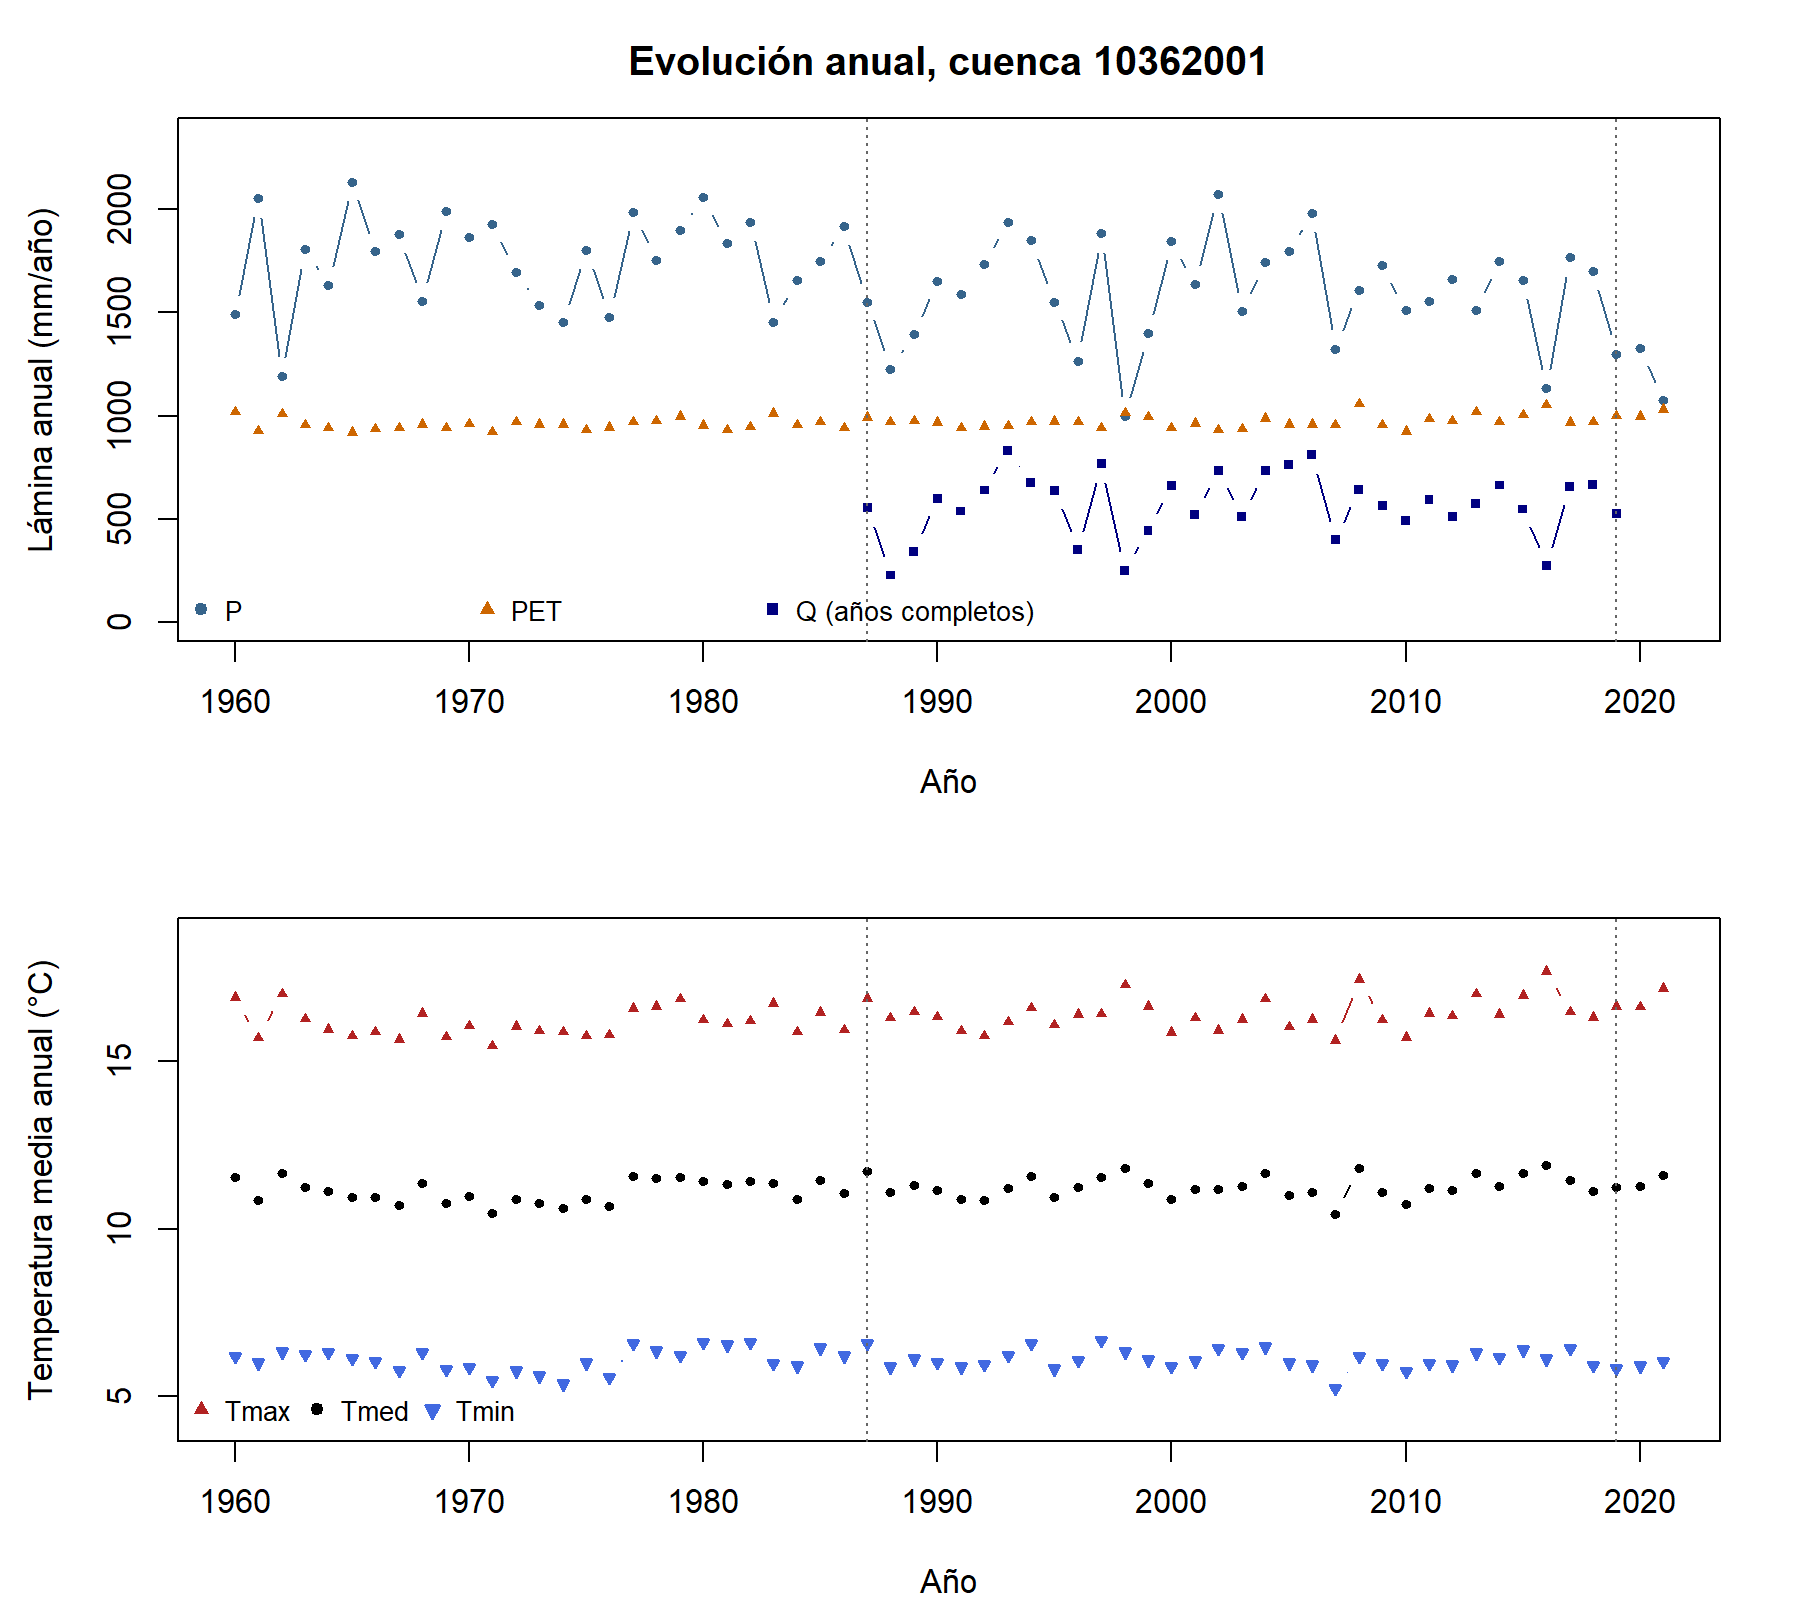
\includegraphics[width=0.9\textwidth]{../03_outputs/figures/05_evolucion_anual.png}}{%
\fbox{Falta 03\_outputs/figures/05\_evolucion\_anual.png}}
\caption{Arriba: P, PET y Q anuales en lámina (mm\,año$^{-1}$). Abajo:
Tmax, Tmed y Tmin anuales (°C). Clima de CR2MET v2.5 \citep{Boisier2023} de
1960 a 2021; caudal DGA rellenado de 1987 a 2019. Las líneas punteadas
marcan el período de análisis.}
\label{fig:E04evolucion}
\end{figure}

\begin{table}[ht]
\centering
\caption{Estadísticos anuales, 1987--2019 (33 años). CV: coeficiente de
variación. Q/P es adimensional.}
\label{tab:E04estadisticos}
\begin{tabular}{|p{0.22\linewidth}|r|r|r|r|r|}
\hline
Variable & Media & Desviación & CV (\%) & Mínimo (año) & Máximo (año) \\
\hline
P (mm\,año$^{-1}$) & 1601.6 & 247.9 & 15.5 & 999.6 (1998) & 2075.6 (2002) \\
\hline
PET (mm\,año$^{-1}$) & 973.4 & 31.1 & 3.2 & 923.6 (2010) & 1057.8 (2008) \\
\hline
Q (mm\,año$^{-1}$) & 566.1 & 157.2 & 27.8 & 226.7 (1988) & 832.1 (1993) \\
\hline
Q medio (m$^3$\,s$^{-1}$) & 8.41 & 2.34 & 27.8 & 3.36 (1988) & 12.37 (1993) \\
\hline
Q/P & 0.35 & 0.06 & 17.0 & 0.18 (1988) & 0.43 (1993) \\
\hline
Tmax (°C) & 16.43 & 0.48 & 2.9 & 15.62 (2007) & 17.69 (2016) \\
\hline
Tmed (°C) & 11.27 & 0.34 & 3.0 & 10.43 (2007) & 11.91 (2016) \\
\hline
Tmin (°C) & 6.11 & 0.29 & 4.7 & 5.24 (2007) & 6.68 (1997) \\
\hline
\end{tabular}
\end{table}

\begin{table}[ht]
\centering
\caption{Los tres años más secos y los tres más húmedos según la P,
1987--2019. P, PET y Q en mm\,año$^{-1}$; Q/P adimensional.}
\label{tab:E04extremos}
\begin{tabular}{|l|l|r|r|r|r|}
\hline
Tipo & Año & P & PET & Q & Q/P \\
\hline
Seco & 1998 & 999.6 & 1013.2 & 248.9 & 0.25 \\
\hline
Seco & 2016 & 1132.4 & 1053.7 & 272.6 & 0.24 \\
\hline
Seco & 1988 & 1227.5 & 970.8 & 226.7 & 0.18 \\
\hline
Húmedo & 1993 & 1938.8 & 952.1 & 832.1 & 0.43 \\
\hline
Húmedo & 2006 & 1984.1 & 958.1 & 810.3 & 0.41 \\
\hline
Húmedo & 2002 & 2075.6 & 932.6 & 733.9 & 0.35 \\
\hline
\end{tabular}
\end{table}

\begin{table}[ht]
\centering
\caption{Relaciones entre variables anuales, 1987--2019 (33 años).}
\label{tab:E04relaciones}
\begin{tabular}{|p{0.55\linewidth}|r|}
\hline
Indicador & Valor \\
\hline
Correlación de P y Q anuales & 0.92 \\
\hline
Correlación de P y PET anuales & $-$0.49 \\
\hline
Correlación de PET y Tmed anuales & 0.72 \\
\hline
P $-$ Q medio, ecuación~(\ref{eq:E04balance}) (mm\,año$^{-1}$) & 1035.4 \\
\hline
PET media (mm\,año$^{-1}$) & 973.4 \\
\hline
(P $-$ Q)/PET & 1.064 \\
\hline
Años con P $-$ Q mayor que la PET & 23 de 33 \\
\hline
Volumen anual que viene de días rellenados, 2016 / 2013 & 45.0 / 44.3 \% \\
\hline
\end{tabular}
\end{table}

\campo{3. Fuente y trazabilidad}{Las series anuales salen de
\texttt{02\_\allowbreak{}Rscripts/\allowbreak{}05\_\allowbreak{}regimen\_\allowbreak{}hidroclimatico.R}, que agrega la serie
diaria de clima de E02 y el caudal rellenado pasado a lámina con el área de
E01 (468.73 km$^2$). Las cifras de esta ficha están en
\texttt{03\_\allowbreak{}outputs/\allowbreak{}tables/\allowbreak{}} (\texttt{05\_\allowbreak{}clima\_\allowbreak{}caudal\_\allowbreak{}anual.csv},
\texttt{05\_\allowbreak{}estadisticos\_\allowbreak{}anuales\_\allowbreak{}E04.csv},
\texttt{05\_\allowbreak{}anios\_\allowbreak{}extremos\_\allowbreak{}E04.csv},
\texttt{05\_\allowbreak{}relaciones\_\allowbreak{}anuales\_\allowbreak{}E04.csv} y
\texttt{05\_\allowbreak{}relleno\_\allowbreak{}por\_\allowbreak{}anio\_\allowbreak{}E04.csv}) y la figura en
\texttt{03\_\allowbreak{}outputs/\allowbreak{}figures/\allowbreak{}05\_\allowbreak{}evolucion\_\allowbreak{}anual.png}. El período se lee de
\texttt{06\_\allowbreak{}config/\allowbreak{}parametros.csv}, las fuentes están en
\texttt{04\_\allowbreak{}metadata/\allowbreak{}data\_\allowbreak{}sources.csv} y todo se regenera con
\texttt{run\_\allowbreak{}all.R}.}

\campo{4. Interpretación hidrológica}{El caudal varía casi el doble que la
lluvia: su coeficiente de variación es 27.8 \%, contra 15.5 \% de la
P. La correlación entre P y Q anuales es 0.92, pero la respuesta no es
proporcional. En los años secos solo entre un 18 y un
25 \% de la P sale como caudal, y en los húmedos llega hasta un
43 \%: con menos lluvia, la parte que se evapora o queda en la
cuenca pesa más. La PET casi no cambia entre años (CV 3.2 \%) y tiende
a ir al revés de la P (correlación $-$0.49): 1998 y 2016, dos de los años
más secos, tienen PET sobre la media, aunque 1988 no. La ecuación de
Hargreaves hace subir la PET con la temperatura y con la diferencia entre
Tmax y Tmin, que está ligada a la nubosidad \citep{Allen1998}. Las
temperaturas varían poco: la Tmed va de 10.43 °C (2007) a
11.91 °C (2016).

En 1987--2019 no se detecta un cambio en P, PET ni Tmed: Pettitt no
encuentra quiebre y el KPSS no rechaza la estacionariedad, aunque el ADF no
la confirma (E02). Las pruebas del integrante 2 tampoco encuentran quiebre en
el caudal. No se aplicó una prueba de tendencia, así que lo defendible es que
no se detecta cambio, no que no lo haya. En el registro largo sí hay cambios:
el de Tmed (desde 1977) es anterior al período, el de P (desde 1987) coincide
con su inicio, y el de PET (desde 2011, +3.8 \%) cae dentro del período, pero
dentro de 1987--2019 no resulta significativo.}

\campo{5. Consistencia física}{Los flujos se suman en el año y las
temperaturas se promedian; los años bisiestos entran con sus 366 días porque
la regla de completitud cuenta los días del calendario. El caudal en lámina
sale de la ecuación~(\ref{eq:E03lamina}) de E03, sumada en el año. Si el
almacenamiento no cambia en el largo plazo, la ET real es lo que queda del
balance:
\begin{equation}
\mathrm{ET}_{\mathrm{real}} \approx P - Q
\label{eq:E04balance}
\end{equation}
Aquí P $-$ Q supera a la PET en un 6.4 \% en promedio y en
23 de los 33 años (Tabla~\ref{tab:E04relaciones}). La PET de
Hargreaves estima la ET de un cultivo de referencia \citep{Allen1998} y no
la de la cobertura real de la cuenca, pero un exceso sostenido indica además
que algún término puede tener un sesgo: la P sobreestimada, el caudal
subestimado (extracciones, pérdidas hacia el acuífero o la curva de
descarga) o la PET subestimada. Se trata en E05 y E06.}

\campo{6. Limitaciones e incertidumbre}{33 años es poco para hablar de
tendencias. En 11 de los 33 años el caudal anual incluye días rellenados
(E02), con bloques de hasta 71 días. En 2016, uno de los años más secos, el
45.0 \% del volumen anual viene de días rellenados, y en 2013 el
44.3 \%, así que el Q/P de esos años depende en buena parte de la
regresión. En 2014 los 15 días rellenados quedaron en 0 y no aportan
volumen. La P, Tmax y Tmin son de un producto grillado y la PET de una
fórmula que usa solo temperatura, así que la relación entre PET y P refleja
también cómo se construyen esas variables.}

\campo{7. Conclusión asociada}{Entre 1987 y 2019 el caudal del Río Damas en
Tacamo varía casi el doble que la lluvia y responde a ella de forma no
proporcional: en los años secos sale como caudal una fracción menor de la P.
En el período no se detecta cambio en P, PET, Tmed ni Q. El balance de largo
plazo deja P $-$ Q por encima de la PET en 23 de 33 años, algo que E05 y E06
tienen que explicar antes de interpretar la ET real.}
